\documentclass[14pt]{extbook}
\usepackage{multicol, enumerate, enumitem, hyperref, color, soul, setspace, parskip, fancyhdr} %General Packages
\usepackage{amssymb, amsthm, amsmath, latexsym, units, mathtools} %Math Packages
\everymath{\displaystyle} %All math in Display Style
% Packages with additional options
\usepackage[headsep=0.5cm,headheight=12pt, left=1 in,right= 1 in,top= 1 in,bottom= 1 in]{geometry}
\usepackage[usenames,dvipsnames]{xcolor}
\usepackage{dashrule}  % Package to use the command below to create lines between items
\newcommand{\litem}[1]{\item#1\hspace*{-1cm}\rule{\textwidth}{0.4pt}}
\pagestyle{fancy}
\lhead{Module6}
\chead{}
\rhead{Version B}
\lfoot{2107-1615}
\cfoot{}
\rfoot{test}
\begin{document}

\begin{enumerate}
\litem{
Construct the lowest-degree polynomial given the zeros below. Then, choose the intervals that contain the coefficients of the polynomial in the form $x^3+bx^2+cx+d$.\[ -4 + 5 i \text{ and } -3 \]\begin{enumerate}[label=\Alph*.]
\item \( b \in [-14, -10], c \in [63, 72], \text{ and } d \in [-129, -116] \)
\item \( b \in [7, 14], c \in [63, 72], \text{ and } d \in [119, 125] \)
\item \( b \in [1, 9], c \in [-5, 1], \text{ and } d \in [-24, -14] \)
\item \( b \in [1, 9], c \in [4, 13], \text{ and } d \in [11, 20] \)
\item \( \text{None of the above.} \)

\end{enumerate} }
\litem{
Construct the lowest-degree polynomial given the zeros below. Then, choose the intervals that contain the coefficients of the polynomial in the form $ax^3+bx^2+cx+d$.\[ \frac{-5}{2}, \frac{-7}{4}, \text{ and } -2 \]\begin{enumerate}[label=\Alph*.]
\item \( a \in [3, 9], b \in [3, 13], c \in [-51, -46], \text{ and } d \in [-70, -67] \)
\item \( a \in [3, 9], b \in [48, 52], c \in [97, 108], \text{ and } d \in [68, 74] \)
\item \( a \in [3, 9], b \in [48, 52], c \in [97, 108], \text{ and } d \in [-70, -67] \)
\item \( a \in [3, 9], b \in [-60, -47], c \in [97, 108], \text{ and } d \in [-70, -67] \)
\item \( a \in [3, 9], b \in [-23, -17], c \in [-33, -29], \text{ and } d \in [68, 74] \)

\end{enumerate} }
\litem{
Describe the zero behavior of the zero $x = 5$ of the polynomial below.\[ f(x) = 2(x - 7)^{10}(x + 7)^{8}(x - 5)^{8}(x + 5)^{3} \]\begin{enumerate}[label=\Alph*.]
\begin{multicols}{2}\item 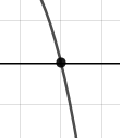
\includegraphics[width = 0.3\textwidth]{../Figures/polyZeroBehaviorAB.png}\item 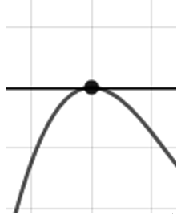
\includegraphics[width = 0.3\textwidth]{../Figures/polyZeroBehaviorBB.png}\item 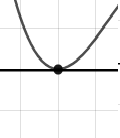
\includegraphics[width = 0.3\textwidth]{../Figures/polyZeroBehaviorCB.png}\item 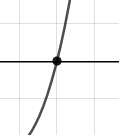
\includegraphics[width = 0.3\textwidth]{../Figures/polyZeroBehaviorDB.png}\end{multicols}\item None of the above.
\end{enumerate} }
\litem{
Describe the zero behavior of the zero $x = 5$ of the polynomial below.\[ f(x) = -4(x + 4)^{8}(x - 4)^{7}(x - 5)^{9}(x + 5)^{4} \]\begin{enumerate}[label=\Alph*.]
\begin{multicols}{2}\item 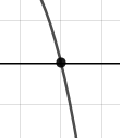
\includegraphics[width = 0.3\textwidth]{../Figures/polyZeroBehaviorCopyAB.png}\item 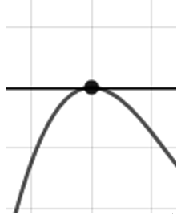
\includegraphics[width = 0.3\textwidth]{../Figures/polyZeroBehaviorCopyBB.png}\item 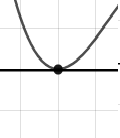
\includegraphics[width = 0.3\textwidth]{../Figures/polyZeroBehaviorCopyCB.png}\item 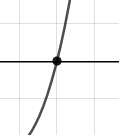
\includegraphics[width = 0.3\textwidth]{../Figures/polyZeroBehaviorCopyDB.png}\end{multicols}\item None of the above.
\end{enumerate} }
\litem{
Which of the following equations \textit{could} be of the graph presented below?
\begin{center}
    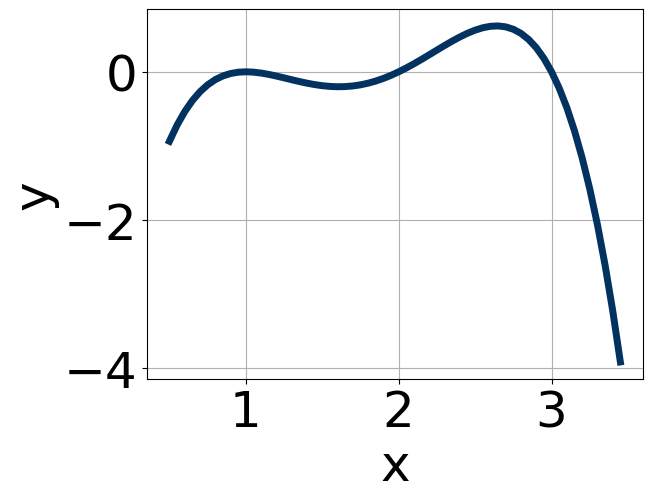
\includegraphics[width=0.5\textwidth]{../Figures/polyGraphToFunctionCopyB.png}
\end{center}
\begin{enumerate}[label=\Alph*.]
\item \( 6(x - 3)^{8} (x - 2)^{7} (x + 4)^{5} \)
\item \( -9(x - 3)^{8} (x - 2)^{10} (x + 4)^{7} \)
\item \( -11(x - 3)^{11} (x - 2)^{5} (x + 4)^{9} \)
\item \( -5(x - 3)^{10} (x - 2)^{7} (x + 4)^{7} \)
\item \( 19(x - 3)^{7} (x - 2)^{9} (x + 4)^{5} \)

\end{enumerate} }
\litem{
Describe the end behavior of the polynomial below.\[ f(x) = 8(x + 8)^{2}(x - 8)^{3}(x + 4)^{5}(x - 4)^{5} \]\begin{enumerate}[label=\Alph*.]
\begin{multicols}{2}\item 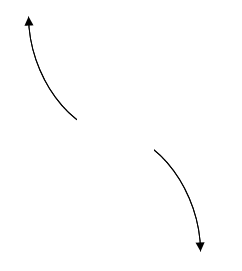
\includegraphics[width = 0.3\textwidth]{../Figures/polyEndBehaviorAB.png}\item 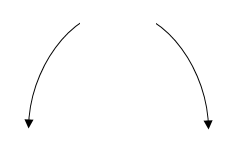
\includegraphics[width = 0.3\textwidth]{../Figures/polyEndBehaviorBB.png}\item 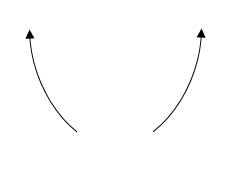
\includegraphics[width = 0.3\textwidth]{../Figures/polyEndBehaviorCB.png}\item 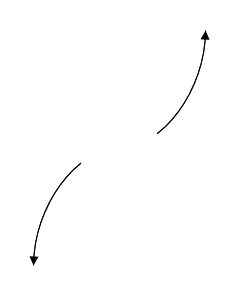
\includegraphics[width = 0.3\textwidth]{../Figures/polyEndBehaviorDB.png}\end{multicols}\item None of the above.
\end{enumerate} }
\litem{
Construct the lowest-degree polynomial given the zeros below. Then, choose the intervals that contain the coefficients of the polynomial in the form $x^3+bx^2+cx+d$.\[ 3 - 5 i \text{ and } -4 \]\begin{enumerate}[label=\Alph*.]
\item \( b \in [0.96, 1.62], c \in [7.42, 9.73], \text{ and } d \in [17, 22] \)
\item \( b \in [-2.98, -1.83], c \in [9.75, 11.93], \text{ and } d \in [132, 142] \)
\item \( b \in [1.06, 2.5], c \in [9.75, 11.93], \text{ and } d \in [-137, -131] \)
\item \( b \in [0.96, 1.62], c \in [0.77, 1.03], \text{ and } d \in [-18, -5] \)
\item \( \text{None of the above.} \)

\end{enumerate} }
\litem{
Construct the lowest-degree polynomial given the zeros below. Then, choose the intervals that contain the coefficients of the polynomial in the form $ax^3+bx^2+cx+d$.\[ 2, \frac{3}{5}, \text{ and } 4 \]\begin{enumerate}[label=\Alph*.]
\item \( a \in [2, 7], b \in [-10, -1], c \in [-54, -35], \text{ and } d \in [-28, -21] \)
\item \( a \in [2, 7], b \in [-38, -29], c \in [54, 63], \text{ and } d \in [-28, -21] \)
\item \( a \in [2, 7], b \in [-38, -29], c \in [54, 63], \text{ and } d \in [19, 31] \)
\item \( a \in [2, 7], b \in [32, 34], c \in [54, 63], \text{ and } d \in [19, 31] \)
\item \( a \in [2, 7], b \in [-18, -8], c \in [-41, -31], \text{ and } d \in [19, 31] \)

\end{enumerate} }
\litem{
Describe the end behavior of the polynomial below.\[ f(x) = 4(x - 6)^{4}(x + 6)^{7}(x + 8)^{5}(x - 8)^{5} \]\begin{enumerate}[label=\Alph*.]
\begin{multicols}{2}\item 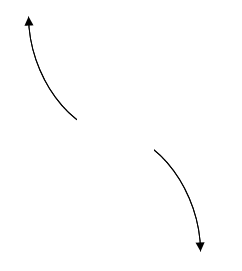
\includegraphics[width = 0.3\textwidth]{../Figures/polyEndBehaviorCopyAB.png}\item 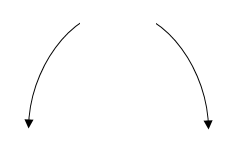
\includegraphics[width = 0.3\textwidth]{../Figures/polyEndBehaviorCopyBB.png}\item 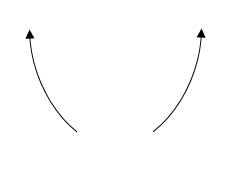
\includegraphics[width = 0.3\textwidth]{../Figures/polyEndBehaviorCopyCB.png}\item 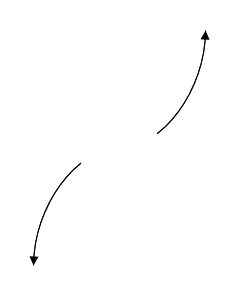
\includegraphics[width = 0.3\textwidth]{../Figures/polyEndBehaviorCopyDB.png}\end{multicols}\item None of the above.
\end{enumerate} }
\litem{
Which of the following equations \textit{could} be of the graph presented below?
\begin{center}
    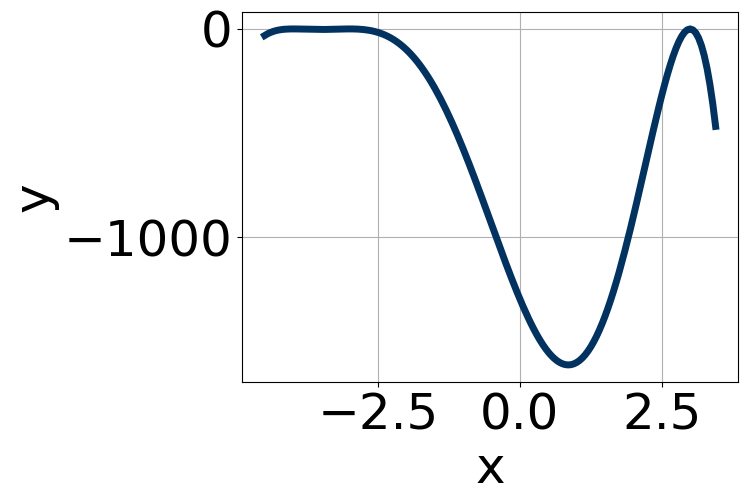
\includegraphics[width=0.5\textwidth]{../Figures/polyGraphToFunctionB.png}
\end{center}
\begin{enumerate}[label=\Alph*.]
\item \( -20x^{9} (x + 2)^{7} (x + 1)^{10} \)
\item \( 14x^{8} (x + 2)^{8} (x + 1)^{9} \)
\item \( -19x^{9} (x + 2)^{4} (x + 1)^{7} \)
\item \( 19x^{5} (x + 2)^{10} (x + 1)^{5} \)
\item \( -18x^{7} (x + 2)^{4} (x + 1)^{10} \)

\end{enumerate} }
\end{enumerate}

\end{document}